\documentclass{article}
\usepackage{graphicx} % Required for inserting images
\usepackage{tikz}
\usepackage{amsmath}
\usepackage{hyperref}
\bibliographystyle{plain}

\title{All you need to know! (ish)}
\author{Laura Midgley }
\date{November 2025}

\begin{document}

\maketitle

\section{Introduction}


\begin{figure}[b!]
    \centering
    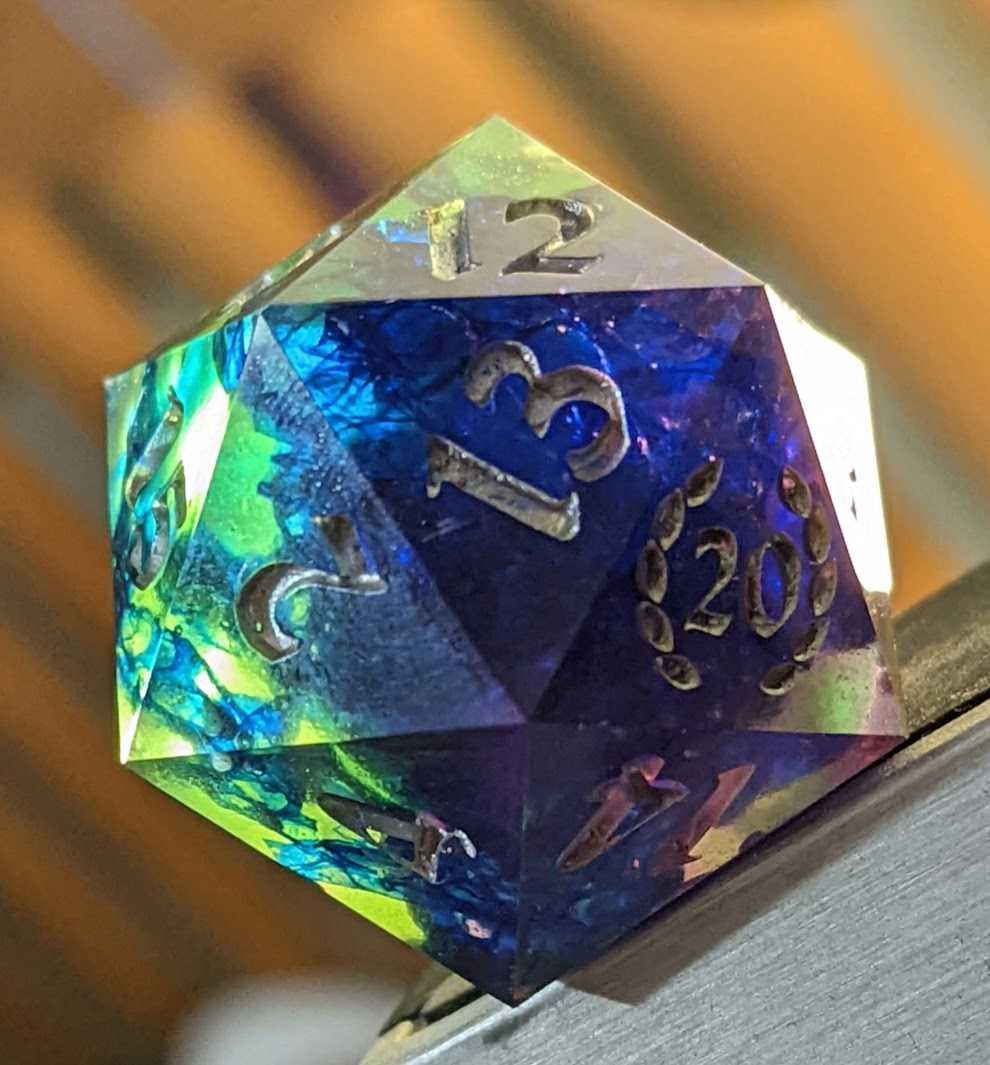
\includegraphics[width=0.5\linewidth]{snakeDice.jpg}
    \caption{Cool dice I made with snake shed}
    \label{fig:snakedice}
\end{figure}

We're going to look at the major components of a \LaTeX document

\section{Mathmode}

To write maths, you need to be in \textit{mathmode}. This lets \LaTeX make your maths mathematically pretty (rather than document-pretty). There's quite a few ways to get into and out of mathmode, but the equation environment will be your first port of call:

\begin{equation}
    a^2+b^2=         c^2 \label{eq:pythag}
\end{equation}

%the place where I interactively write out an equation
%let's make the equation a^2+b^2=c^2, as a nice easy example!

$$\int^\infty_0 x^k dx$$

Another example is the use of \$! Single \$ are used for \textit{inline} equations, whilst \$\$ is a shorthand for the equation mode above without numbers!

This is my cool equation $\tan(\theta)=\frac{\sin(\theta)}{\cos(\theta)}$.
%Write an inline equation here! Let's put a fraction in, and some symbols - maybe tan = sin/cos?

Make sure you always begin \textit{and} end an equation, or else your text will be all squished together after. You can reference an equation like the Equation above %\eqref{eq:pythag} 
 using the \texttt{\textbackslash eqref} command.

In equation \eqref{eq:pythag} we see Pythagoras' theorem.
 

%note to self - trying to use eqref should hit us onto the amsmath package usage


\section{Images}

You'll probably need to put images or figures in your document, so we'll do that here! I already have a picture uploaded in the `file structure' to the left.


%note to self - start begin figure and then let overleaf fill it in!
%use package - graphicx

You can reference with the \texttt{\textbackslash ref} command, for example ``Figure \ref{fig:snakedice} demonstrates the effectiveness of putting different materials within dice."

%use 'hyperref' at this point!


You might need to draw things, so we're also going to look at a tikz picture. Much of Figure \ref{fig:tikzExample} is pre-made, and we're just going to make a few edits and look at the structure.
\begin{figure}
\begin{center}
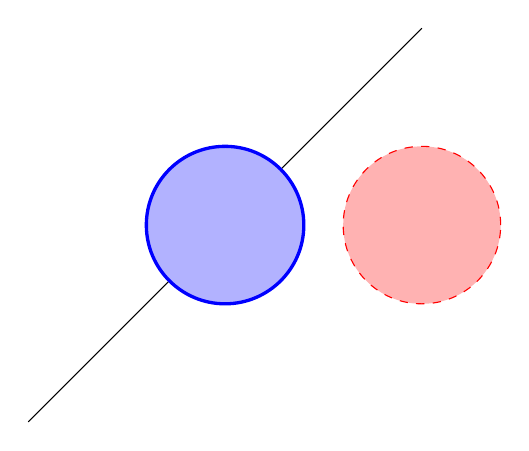
\begin{tikzpicture}
    \draw[-] (0,0) -- (5,5);
    \filldraw[color=blue,fill=blue!30, very thick] (2.5,2.5) circle (1);
    \filldraw[color=red,fill=red!30, dashed] (5,2.5) circle (1);
\end{tikzpicture}
\caption{some shapes made with tikz}
\label{fig:tikzExample}
\end{center}
\end{figure}

We can also look at image positioning here - the `htbp' positioning declarations to bias the image location. You are very unlikely to be able to put an image precisely where you want it pixel-wise, so you may have to accept `latex knows best'!

\section{Table}

\begin{table}[]
    \centering
    \begin{tabular}{l|||c|cr}
    title & title & woah & title \\ \hline
        1 &2  &3&4\\
        left & center & center & right 
    \end{tabular}
    \caption{Caption}
    \label{tab:placeholder}
\end{table}

\section{Bibliography}

It's really important to let people know where you got information from, for a variety of reasons including but not limited to:
\begin{itemize}
    \item so they can read further
    \item so they can check something which doesn't make sense
    \item to give credit where it is due
    \item so you're not pretending you came up with an idea when you got it from elsewhere
    \item to leave a clear line of the history of your studies
    \item so \textit{you} can go back and look at it later
\end{itemize}

I \textit{highly} recommend keeping track of \textit{everything} you read as you go along - and for that, you'll want to grab references and add them to your references.bib (any template I provide you will have this!). When you want to reference something you use the \texttt{\textbackslash cite} command.

As we can see in \cite{reich2020failure} tech is not always the answer.

\bibliography{references} 

\end{document}
